\documentclass{article}
\usepackage{graphicx} % Required for inserting images
\usepackage{hyperref}
\usepackage{amsmath}
\usepackage{amssymb}
\usepackage{algorithm}
\usepackage{algpseudocode}
\usepackage{tabularx}
\usepackage{bm}
\usepackage{multirow}

\usepackage[left=1in, right=1in, top=1in, bottom=1in]{geometry}


\title{
    \hrulefill \\
    \vspace{0.5cm}
    \textbf{FORD-FULKERSON ALGORITHM} \\
    \vspace{0.5cm}
    \hrulefill
    \vspace*{1cm}
}
\author{
\textbf{Tamim Hasan Saad} \\Student ID: 2005095\\ \textbf{Habiba Rafique} \\Student ID: 2005096 \\ 
\textbf{Sadia Afrin Sithi} \\Student ID: 2005119
\vspace*{1cm}
}

\date{
CSE-300:Technical Writing and Presentation\\
Department of Computer Science and Engineering\\
Bangladesh University of Engineering and Technology\\
\vspace*{1cm}
\today
}

\begin{document}
\pagenumbering{roman} 
\maketitle
\pagebreak
\tableofcontents
\pagebreak
\listoffigures
\pagebreak
\listoftables


\clearpage
\pagenumbering{arabic} % Switch to Arabic numbering for the main content

\section{\textbf{INTRODUCTION}}
{\fontsize{15}{15}\selectfont
The Ford-Fulkerson algorithm is a classic method for computing the maximum flow in a flow network, which is a directed graph where each edge has a capacity and represents a pathway through which a material (or flow) can travel from a source node to a sink node. This algorithm iteratively finds augmenting paths from the source to the sink and increases the flow along these paths until no more augmenting paths can be found.
}

\vspace{0.7cm}

\section{\textbf{FORD FULKERSON METHOD}}
{\fontsize{15}{15}\selectfont
The Ford–Fulkerson method or Ford–Fulkerson algorithm (FFA) is a \textbf{greedy algorithm} that computes the maximum flow in a flow network. It is called a "method" instead of an "algorithm" as the approach to finding augmenting paths in a residual graph is not fully specified or it is specified in sev-eral implementations with different running times. It was pub-lished in 1956 by \textbf{L.R. Ford Jr.} and \textbf{Dr. Fulkerson}. The name "Ford–Fulkerson" is often also used for the Edmonds-Karp algorithm, which is a specialization of Ford–Fulkerson. The idea behind the algorithm is as follows: as long as there is a path from the source (start node) to the sink (end node), with available capacity on all edges in the path, we send flow along one of the paths. Then we find another path, and so on. A path with available capacity is called an augmenting path. \\

\vspace{0.3cm}
The Ford-Fulkerson algorithm particularly has a lot of applica-tions. Some of them are:
\begin{itemize}
    \item Network Traffic Optimization
    \item Water Distribution Systems
    \item Electric Power Grids
    \item Airline scheduling
    \item stereo cor-respondence etc.
\end{itemize}
\vspace{0.3cm}
where the given problem is transformed into a maximum flow minimum cut problem and then solved us-ing the Ford-Fulkerson algorithm.
}
\cite{cormen2001section}
\pagebreak

\subsection{\textbf{ DEFINTIONS AND CONCEPTS}}
\vspace{0.5cm}
{\fontsize{15}{15}\selectfont
\begin{enumerate}
    \item \textbf{Flow Network}
    \begin{itemize}
        \item  A flow network is a directed graph G = (V,E) where each edge (u,v) has a non-negative capacity c(u,v), representing the maximum flow that can pass through that edge.
    \end{itemize}
    \vspace{0.7cm}
    
    \item \textbf{Flow} 
    \begin{itemize}
         \item A flow in a network is a function \( \bm{f: V \times V \rightarrow \mathbb{R} }\) that satisfies the properties:
        \( \bm{0 \leq f(u, v) \leq \c(u, v)} \) for all \( (u, v) \) in \( E \) known as \textbf{Capacity constraint} and 
         For every node \( \bm{v \in V - \{s, t\}} \), the total incoming flow is equal to the total outgoing flow: \( \bm{\sum_{u \in V} f(u, v) = \sum_{w \in V} f(v, w)} \) known as \textbf{Flow conservation}.
    \end{itemize}
    \vspace{0.7cm}

    \item \textbf{Maximum Flow}
    \begin{itemize}
        \item  Maximum flow is the maximum amount of flow that can be sent from the source node s to the sink node t in the flow network.
        \item It is achieved when no more augmenting paths can be found in the residual graph.
        \item The flow obtained using the Ford-Fulkerson algorithm is considered the maximum flow for the given network.
    \end{itemize}
    \vspace{0.7cm}

    \item \textbf{Residual Graph}
    \begin{itemize}
        \item A residual graph is a modified version of the original flow network graph.
        \item It reflects the remaining capacity on each edge after some flow has been pushed through.
        \item In the residual graph:
        \begin{itemize}
            \item If the original edge has capacity $c(u,v)$ and flow $f(u,v)$, the residual capacity of the edge is \( \bm{c(u,v) - f(u,v)} \).
            \item If there's a reverse edge in the original graph (to allow backflow), with flow $f(v,u)$, the residual capacity of this edge is \(\bm{f(v,u)}\).
        \end{itemize}
        \item Residual graphs are used to find augmenting paths efficiently in the Ford-Fulkerson algorithm.
    \end{itemize}
    \vspace{0.7cm}
        \begin{figure}
        \centering
        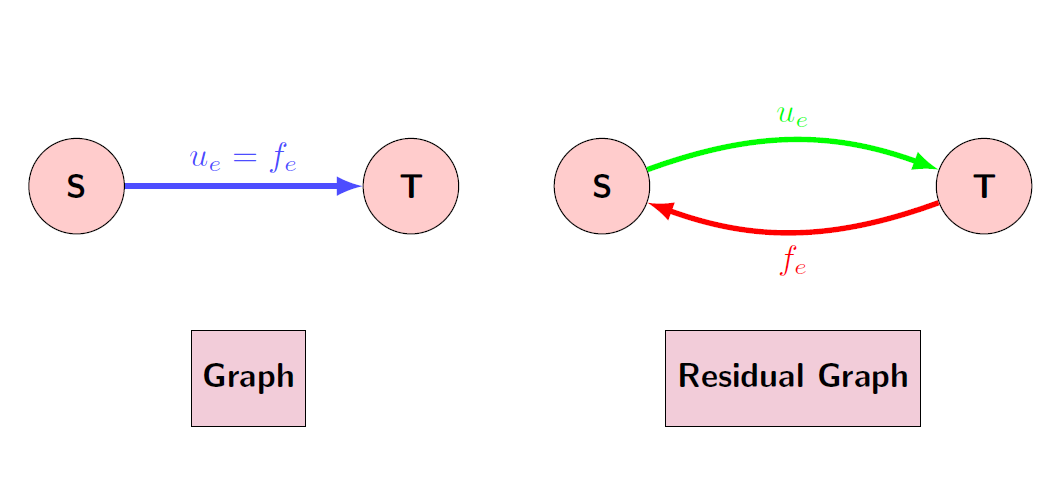
\includegraphics[height = 8cm, width = 12cm]{images/Residual.png}
        \caption{Residual Graph}
        \label{fig:residual}
    \end{figure}
    
    \vspace{0.7cm}
    \item \textbf{Augmenting Path}
    \begin{itemize}
       \item An augmenting path is a simple path from the source node \( s \) to the sink node \( t \) in the residual graph.
       \item Residual graph is a modified version of the original graph that reflects the remaining capacity on each edge after the flow has been pushed through some paths.
       \item An augmenting path allows us to increase the flow from the source to the sink.
       \item When no augmenting path exists, the flow obtained is considered maximum.
    \end{itemize}
    \vspace{0.7cm}
    
    \begin{figure}
        \centering
        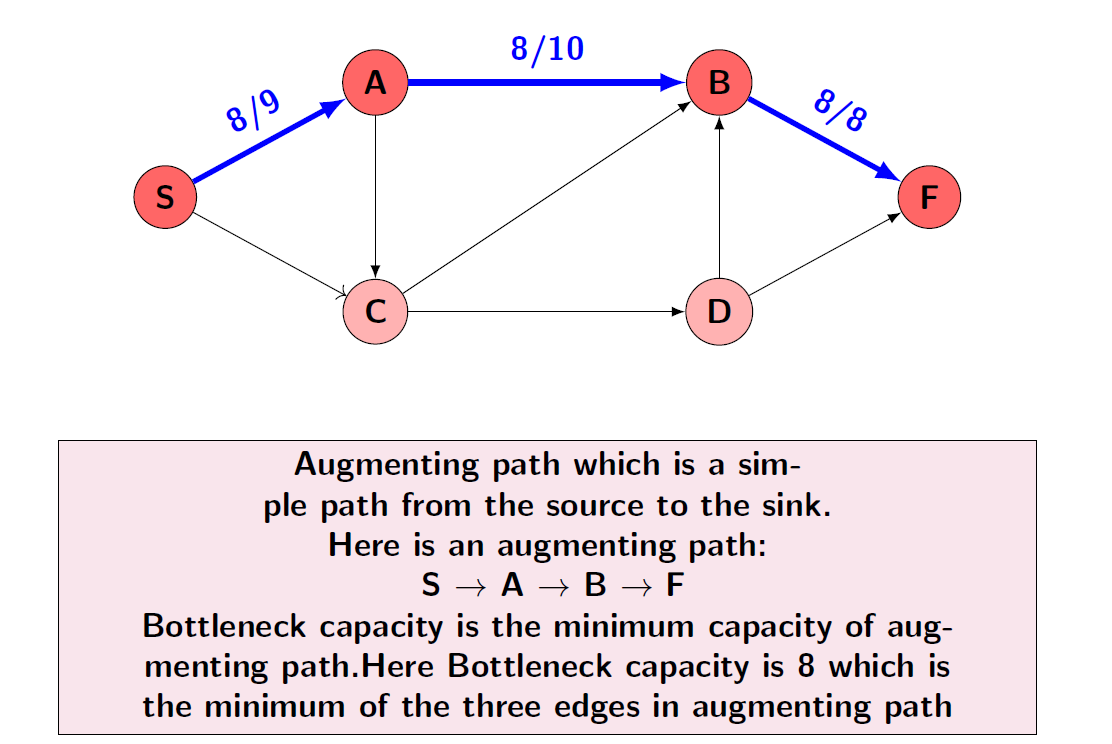
\includegraphics[height = 10cm, width = 14cm]{images/augment.png}
        \caption{Augmenting Path and Bottleneck Capacity}
        \label{fig:augmenting path}
    \end{figure}
    
    \item \textbf{Bottleneck Capacity}
    \begin{itemize}
        \item The bottleneck capacity of an augmenting path is the minimum capacity among all the edges in that path.
        \item It determines the maximum amount of flow that can be pushed through the augmenting path.
        \item When augmenting the flow along a path, the bottleneck capacity limits the amount of flow that can be increased.
        \item The bottleneck capacity is crucial in determining the maximum flow through the network.
    \end{itemize}
    \vspace{0.6cm}
    \end{enumerate}
    
    \vspace{1cm}
    
These definitions provide a basic understanding of the key elements involved in the Ford-Fulkerson algorithm for computing maximum flow in a flow network.
\pagebreak
\vspace{1cm}
\subsection{\textbf{PROBLEM SPECIFICATION}}
{\fontsize{15}{15}\selectfont
Given a flow network represented by a directed graph G = (V,E) with a source node s, a sink node t, and capacities c(u,v) on each edge $(u,v) \in E$, the Ford-Fulkerson algorithm aims to find the maximum possible flow from the source s to the sink t while respecting the capacity constraints of the edges.

\vspace{0.6cm}
More formally, the problem can be stated as follows:

\vspace{0.3cm}
\begin{enumerate}
    \item \textbf{Input}
    \begin{itemize}
        \item A directed graph G = (V,E) representing the flow network.
        \item Source node s and sink node t in V.
        \item Capacities c(u,v) for each edge $(u,v) \in E$, indicating the maximum flow that can traverse that edge.
    \end{itemize}
    \item \textbf{Output} 
    \begin{itemize}
        \item A flow function f that assigns a flow value to each edge $(u,v) \in E$, such that:
   
    \begin{enumerate}
        \item \textbf{Capacity constraint:} $0 \leq f(u,v) \leq c(u,v)$ for all $(u,v) \in E$. 
        \item \textbf{Flow conservation:} For every node $v \in V - \{s,t\}$, the total incoming flow is equal to the total outgoing flow:\\
        \begin{center}
        \[\sum_{u \in V} f(u,v) = \sum_{w \in V} f(v,w)\]
        \end{center}
    \end{enumerate}
    \vspace{0.5cm}
    \item The maximum flow value, which represents the total amount of material that can be transported from s to t in the network.
    \end{itemize} 
\end{enumerate}

\vspace{0.5cm}
The Ford-Fulkerson algorithm iteratively finds augmenting paths from s to t and increases the flow along these paths until no more augmenting paths exist. An augmenting path is a simple path from s to t in the residual graph (a modified version of the original graph that reflects the remaining capacity on each edge). When no more augmenting paths can be found, the algorithm terminates, and the flow obtained is the maximum flow.
}\cite{kleinberg2006algorithm}
\pagebreak
\section{\textbf{FORD-FULKERSON ALGORITHM}}
\vspace{0.5cm}
\subsection{\textbf{ALGORITHM DESCRIPTION}}
{\fontsize{15}{15}\selectfont 
Let $G(V,E)$ be a graph, and for every edge from $u$ to $v$ let $c(u,v)$ be the capacity and $f(u,v)$ be the flow. We want to find the maximum flow from the source $s$ to sink $t$. After every step in the algorithm, the following conditions are maintained:
\vspace{0.5cm}

\begin{itemize}
    \item The flow along an edge cannot exceed its capacity.
    \item The net flow from $u$ to $v$ must be the opposite of the net flow from $v$ to $u$.
    \item That is, unless $u$ is $s$ or $t$, the net flow to a node is zero except for the source which produces the flow and the sink, which consumes flow.
    \item The flow leaving from $s$ must be equal to the one arriving at $t$.
    \item \textbf{Capacity Constraints:} $\forall (u,v) \in f(u,v) \leq c(u,v)$
    \item \textbf{Skew Symmetry:} $\forall (u,v) \in f(u,v) = -f(u,v)$
    \item \textbf{Flow Conservation:} $\forall u \in V : u \neq s$ and $u \neq t, \sum_{w \in V} f(u, w) = 0$, (where $w \in v$)
    \item \textbf{Value($f$):} $\sum f(s,u) = \sum f(v,t)$ where $s,u,v,t \in E$
\end{itemize}
\vspace{0.5cm}
This means that the flow through the network is a legal flow after each round in the algorithm.
\vspace{0.7cm}
We define the residual network $G_f(V,E_f)$ to be the network with capacity $c_f(u,v) = c(u,v) - f(u,v)$. Notice that it can happen that a flow from $v$ to $u$ is allowed in the residual network, though not allowed in the original network:

\begin{align*}
    \text{If } f(u,v) > 0 \text{ and } c(u,v) = 0, \\
    \text{then } c_f(v,u) &= c(v,u) - f(v,u) \\
                           &= f(u,v) > 0.
\end{align*}
\pagebreak

The basic algorithm is as follows:\\

\vspace{0.2cm}
\textbf{Repeat: find an augmenting path, and augment!}
\vspace{0.4cm}

\begin{algorithm}
\caption{Ford-Fulkerson Algorithm}
\begin{algorithmic}[1]
\State For each edge $(u,v) \in G.E$, $f(u,v) = 0$.
\While{there exists a path $p$ from $s$ to $t$ in the residual network}
    \State $c_f(p) = \min\{c_f(u,v) : (u,v) \text{ is in } p\}$
    \For{each edge $(u,v) \in p$}
        \State $f(u,v) = f(u,v) + c_f(p)$ \Comment{Send flow along the path}
        \State $f(v,u) = f(v,u) - c_f(p)$ \Comment{The flow might be returned later}
    \EndFor
\EndWhile
\end{algorithmic}
\end{algorithm}

\vspace{0.7cm}
The path in the while loop can be found with a breadth-first or depth-first search in $G_f(V,E_f)$. When the former is used, the algorithm is called Edmonds-Karp algorithm.

\vspace{0.5cm}
When no more paths in the while loop can be found, $s$ will not be able to reach $t$ in the residual network. If $S$ is the set of nodes reachable by $s$ in the residual network, then the total capacity in the original network of edges from $S$ to the remainder of $V$ is, on the one hand, equal to the total flow we found from $s$ to $t$, and on the other hand, serves as an upper bound for all such flows. This proves that the flow found is maximal.
}

\pagebreak
\subsection{\textbf{FLOW-CHART}}
\label{sec:flowchart}
\begin{figure}[htbp]
    \centering
    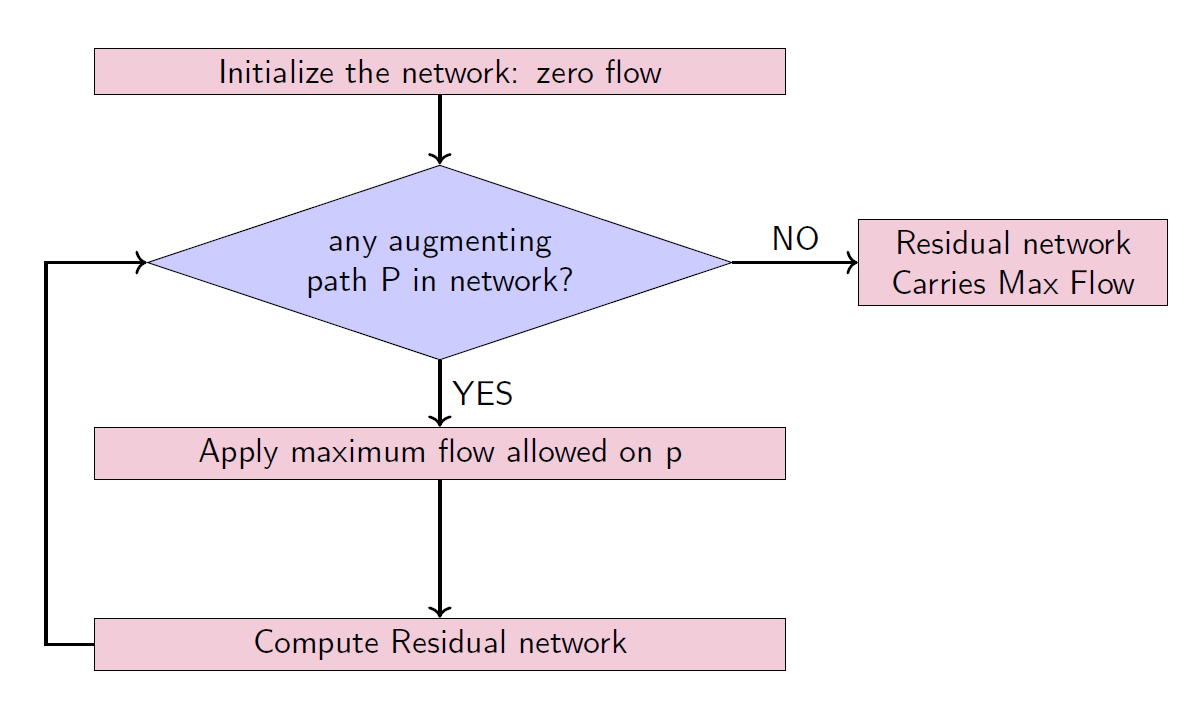
\includegraphics[height = 15cm, width = 17cm]{images/flowchart.png}
    \caption{Flowchart depicting the Ford-Fulkerson algorithm.}
    \label{fig:flowchart}
\end{figure}
\pagebreak

\section{EXAMPLE}

The following example shows the first steps of Ford Fulkerson in a flow network with 6 nodes, source S, sink F.\\
\vspace{0.6cm}
\begin{table}[h]
    \centering
    \begin{tabular}{|c|c|c|}
    \hline
    \textbf{PATH} & \textbf{CAPACITY} & \textbf{RESULTING NETWORK} \\
    \hline
    \multirow{7}{*}{Initial Network} & & \multirow{7}{*}{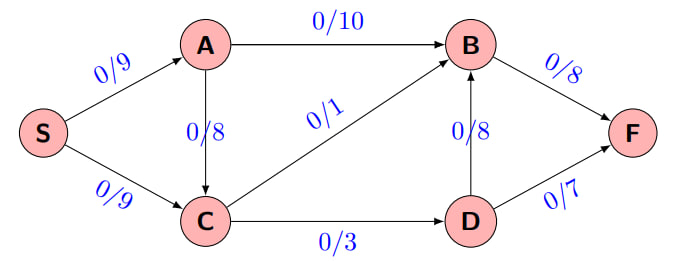
\includegraphics[width=6cm,height=2.5cm]{images/graph0.jpg}} \\
    & & \\
    & & \\
    & & \\
    & & \\
    & & \\
    & & \\
    \hline
    \multirow{7}{*}{S,A,B,F} & $min(c_f(S,A), c_f(A,B), c_f(B,F))$ & \multirow{7}{*}{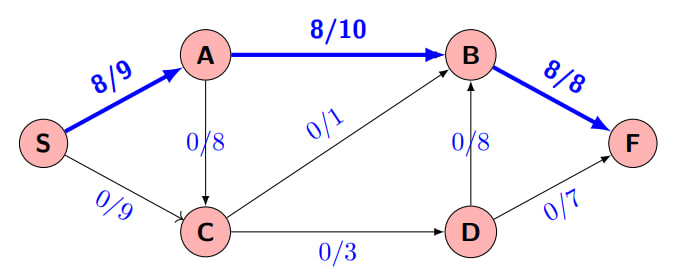
\includegraphics[width=6cm,height=2.5cm]{images/graph1.jpg}} \\
    & & \\
    & & \\
    & & \\
    & & \\
    & $=min(c(S,A)-f(S,A),c(A,B)-$ & \\
    & $f(A,B),c(B,F)-f(B,F))$ & \\
    & & \\
    & $=min(9-0, 10-0, 8-0) = 8$ & \\
    \hline
    \multirow{7}{*}{S,C,D,F} & $min(c_f(S,C), c_f(C,D), c_f(D,F))$ & \multirow{7}{*}{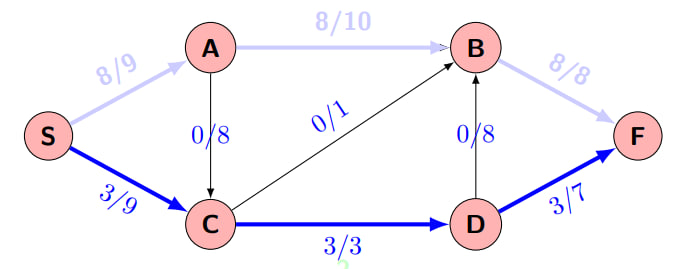
\includegraphics[width=6cm,height=2.5cm]{images/graph2.jpg}} \\
    & & \\
    & & \\
    & & \\
    & & \\
    & $=min(c(S,C)-f(S,C),c(C,D)-$ & \\
    & $f(C,D),c(D,F)-f(D,F))$ & \\
    & & \\
    & $=min(9-0, 3-0, 7-0) = 3$ & \\
    \hline
    \multirow{7}{*}{Resulting network} & & \multirow{7}{*}{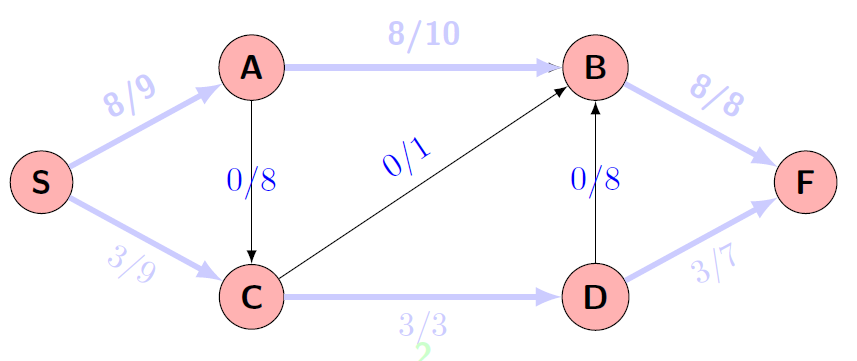
\includegraphics[width=6cm,height=2.5cm]{images/graph3.png}} \\
    & & \\
    & & \\
    & & \\
    & & \\
    & & \\
    & & \\
    \hline
    \end{tabular}
    \caption{Relation between path, capacity, and Resulting Flow Network}
    \label{tab:my_label}     
\end{table}

\pagebreak
\section{\textbf{MAXFLOW-MINCUT}}
\vspace{0.5cm}
\subsection{\textbf{MIN-CUT}}
{\fontsize{15}{15}\selectfont
Min-cut is the one with the minimum total capacity. It has the smallest sum of capacities among all cuts that separate the source and sink nodes.\\
The value of the minimum cut is equal to the maximum flow in the network, which is a fundamental property exploited by the Ford-Fulkerson algorithm for finding the maximum flow.}

\vspace{0.7cm}
\subsection{\textbf{MAXFLOW-MINCUT THEOREM}}
{\fontsize{15}{15}\selectfont
If f is a flow in a flow network G = (V,E), with source s and sink t, then the following conditions are equivalent:\\
\begin{itemize}
    \renewcommand{\labelitemi}{$\Rightarrow$}
    \item f is a maximum flow in G.
    \item The residual network $G_f$ contains no augmented paths.
    \item $|f| = c(S,T)$ for some cut (S,T) (a min-cut).
\end{itemize}
\vspace{0.3cm}
It is a flow since there is no augmented paths It is maximum since the sink is not reachable from the source.}


\label{sec:minCut}
\begin{figure}[htbp]
    \centering
    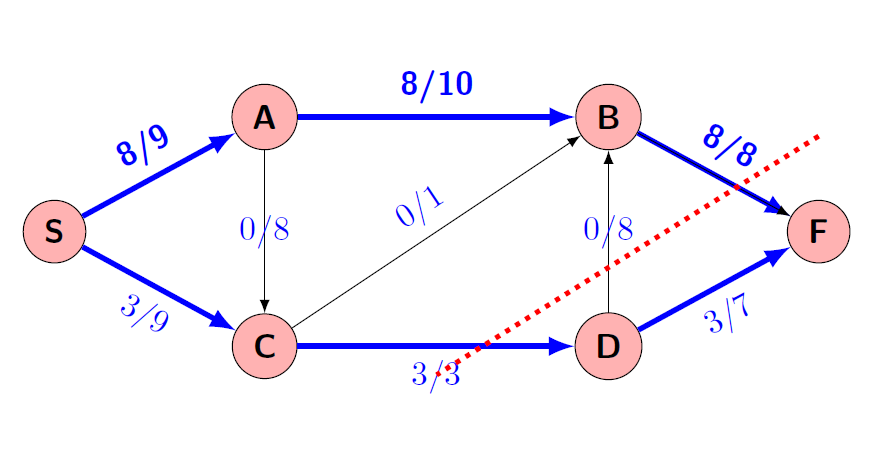
\includegraphics[height = 7cm, width = 8cm]{images/maxMin.png}
    \caption{Maxflow-Mincut Algorithm.}
    \label{fig:minCut}
\end{figure}

\pagebreak

\section{ANALYSIS}
{\fontsize{15}{15}\selectfont
The efficiency of the \textbf{Ford-Fulkerson algorithm} heavily relies on how the augmenting paths \textbf{p} are chosen. Poor choices can lead to non-termination or failure to converge to the maximum flow value.\\

\vspace{0.2cm}
This issue is particularly pronounced when dealing with irrational capacities. In practice, the maximum-flow problem often involves integral capacities, and if they're rational, they can be scaled to integers without loss of generality. In the transformed network with integral capacities, denoted by \textbf{f*}, where\textbf{ f*} represents the \textbf{maximum flow}, a basic implementation of Ford-Fulkerson executes the while loop (lines 2-8) at most \textbf{$\lvert f^* \rvert$} times. This is because the flow value increases by at least one unit in each iteration. \\

\vspace{0.2cm}
For graphs with integral capacities, the runtime of Ford-Fulkerson is bounded by \textbf{O(Ef)}, where E is the number of edges and f is the maximum flow. However, in the presence of irrational values, the flow may fail to converge towards the maximum value, leading the algorithm to run indefinitely.}
\vspace{1cm}

\section{RUNNING TIME}
\textbf{Complexities:}
\begin{itemize}
    \item Residual path: $O(m+n)$
    \item Compute bottleneck capacity: $O(m)$
    \item Update flow: $O(m)$
    \item Update residual graph: $O(m)$
\end{itemize}
\vspace{0.4cm}
\textbf{Total running time:}
\[
O(C(m+n))
\]
\pagebreak

\section{CONCLUSION}
\vspace{0.5cm}
\subsection{\textbf{SUMMARY}}
{\fontsize{15}{15}\selectfont
We have discussed the \textbf{Ford-Fulkersion} method for maximum flow and minimum cut and analysed it's algorithm.Ford-Fulkerson algorithm is a versatile tool with numerous real-world applications in optimizing flow management across various domains.In essence, the Ford-Fulkerson algorithm is a pivotal tool in network optimization, renowned for its versatility and effectiveness in efficiently managing flow and resource allocation across various real-world applications.}

\vspace{0.5cm}
\subsection{\textbf{STRENGTHS AND WEAKNESS}}
{\fontsize{15}{15}\selectfont
\begin{itemize}
    \item The Ford-Fulkerson algorithm possesses several strengths that make it a valuable tool in various optimization problems. Firstly, its versatility allows it to be applied to a wide range of flow network scenarios, including transportation systems, network routing, and resource allocation. Additionally, the algorithm's ability to handle both integral and rational capacities makes it adaptable to real-world scenarios where flow capacities may vary. Moreover, its iterative approach ensures that it converges to the maximum flow solution efficiently, particularly in networks with integral capacities.
    \item However, despite its strengths, the Ford-Fulkerson algorithm has some limitations. One significant weakness is its reliance on finding augmenting paths, which may lead to non-termination or slow convergence, especially in networks with irrational capacities. Additionally, the algorithm's performance can be impacted by the choice of path selection strategy, as poor choices may result in suboptimal solutions or prolonged runtime. Overall, while the Ford-Fulkerson algorithm offers a powerful framework for solving maximum flow problems, its effectiveness can be influenced by the specific characteristics of the flow network and the implementation choices made during execution.
\end{itemize}
}
\pagebreak

\vspace{1cm}
\section{ACKNOWLEDGEMENT}
{\fontsize{15}{15}\selectfont
We would like to express our sincere gratitude to the Department of Computer Science and Engineering of Bangladesh University Of Engineering and Technology for their unwavering support and encouragement throughout the duration of this semester. Their guidance and resources have been instrumental in our endeavors, enabling us to delve into the complexities with confidence and diligence.}


\vspace{0.5cm}
\bibliographystyle{plain}
\bibliography{Bibliography/ref}
\end{document}
